
On considère la série statistique donnée par le tableur ci-dessous. On déterminera à l'aide des questions posées la moyenne et l'écart type de cette série.

\begin{center}
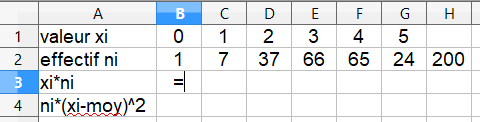
\includegraphics[scale=1]{stat-33.png}
\end{center}


\begin{enumerate}
\item A qui correspond la valeur 200 ? Comment l'obtenir ?
\item Quelle formule faut-il entrer en \textbf{B3} puis étirer vers la droite ?
\item Quelle formule faut-il entrer en \textbf{H3} pour obtenir la moyenne de la série ?
\item Quelle formule faut-il entrer en \textbf{B4} puis étirer vers la droite ?
\item Comment obtenir l'écart type en \textbf{H4} ?
\item Créer ce fichier pour tester vos réponses.
\end{enumerate} 